% Created 2019-07-11 Thu 14:49
% Intended LaTeX compiler: pdflatex
\documentclass[11pt]{article}
  \usepackage[top=0.85in,left=2.75in,footskip=0.75in,marginparwidth=2in]{geometry}

% use Unicode characters - try changing the option if you run into troubles with special characters (e.g. umlauts)
\usepackage[utf8]{inputenc}

% clean citations
\usepackage{cite}

% use \textcolor{color}{text} for colored text (e.g. highlight to-do areas)
\usepackage{xcolor}

% hyperref makes references clicky. use \url{www.example.com} or \href{www.example.com}{description} to add a clicky url
\usepackage{nameref,hyperref}
\hypersetup{backref=true,       
    pagebackref=false,               
    hyperindex=true,                
    colorlinks=true,                
    breaklinks=true,                
    urlcolor= black,                
    linkcolor= blue,                
    bookmarks=true,                 
    bookmarksopen=false,
    filecolor=black,
    citecolor=blue,
    linkbordercolor=blue
}
% line numbers
\usepackage[right]{lineno}

% improves typesetting in LaTeX
\usepackage{microtype}
\DisableLigatures[f]{encoding = *, family = * }

% text layout - change as needed
\raggedright
\setlength{\parindent}{0.25cm}
\textwidth 5.25in 
\textheight 8.75in

% use adjustwidth environment to exceed text width (see examples in text)
\usepackage{changepage}

% adjust caption style
\usepackage[aboveskip=1pt,labelfont=bf,labelsep=period,singlelinecheck=off]{caption}

% remove brackets from references
\makeatletter
\renewcommand{\@biblabel}[1]{\quad#1.}
\makeatother

% headrule, footrule and page numbers
\usepackage{lastpage,fancyhdr,graphicx}
\usepackage{epstopdf}
\pagestyle{myheadings}
\pagestyle{fancy}
\fancyhf{}
\rfoot{\thepage}
\renewcommand{\footrule}{\hrule height 2pt \vspace{2mm}}
\fancyheadoffset[L]{2.25in}
\fancyfootoffset[L]{2.25in}


% define custom colors (this one is for figure captions)
\definecolor{Gray}{gray}{.25}

% this is required to include graphics
\usepackage{graphicx}

% use if you want to put caption to the side of the figure - see example in text
\usepackage{sidecap}

% use for have text wrap around figures
\usepackage{wrapfig}
\usepackage[pscoord]{eso-pic}
\usepackage[fulladjust]{marginnote}
\reversemarginpar

% helvetica font
\usepackage[scaled]{helvet} % Helvetica font (equivalent to Arial)
\renewcommand*\familydefault{\sfdefault} % Helvetica font
\usepackage[T1]{fontenc}

% add garbage text to test formatting
\usepackage{lipsum}
\usepackage{lineno}
\setcounter{secnumdepth}{0}
\author{David R. Hill}
\date{\today}
\title{}
\begin{document}

% title goes here:
\begin{flushleft}
{\huge
  \textbf{
    \newline{The title of the manuscript goes here}
    }
  }
\newline
% authors go here:
\\
David R. Hill\textsuperscript{1,*},
Author 2\textsuperscript{2},
Author 3\textsuperscript{1},
Author 4\textsuperscript{1},
Author 5\textsuperscript{2},
Author 6\textsuperscript{2},
Author 7\textsuperscript{1,*}
\\
\bigskip
1 Division of Gastroeneterology and Hepatology, Department of Internal Medicine, University of Michigan
\\
2 Affiliation B
\\
\bigskip
$\ast$ Corresponding author: hilldr@med.umich.edu

\end{flushleft}

\section*{{\bfseries\sffamily } Abstract}
\label{sec:org797cb99}
Abstract text. \lipsum[4]
\section*{{\bfseries\sffamily } Introduction}
\label{sec:orgf45a75d}
In the introduction, I will in all likelihood need to cite this paper \cite{Hill:2017}. \lipsum
\section*{{\bfseries\sffamily } Materials and Methods}
\label{sec:org58380cd}
\subsection*{{\bfseries\sffamily } Cell Culture}
\label{sec:org37dcf96}
Here I discuss how I grew the cells. \lipsum[2]
\subsection*{{\bfseries\sffamily } Statistical analysis}
\label{sec:org81cf2eb}
A P-value of < 0.05 was considered statistically significant. \lipsum[3]
\section*{{\bfseries\sffamily } Results}
\label{sec:org116bd85}
\subsection*{{\bfseries\sffamily } Figure 1 Standard floating figure}
\label{sec:orgd7ac78a}
Say something interesting about the figure. \lipsum[1-2]
\begin{figure}[ht] % state preferences regarding figure placement (here, top-of-page)
% use to correct figure counter if necessary
%\renewcommand{\thefigure}{2}
  %\centering
  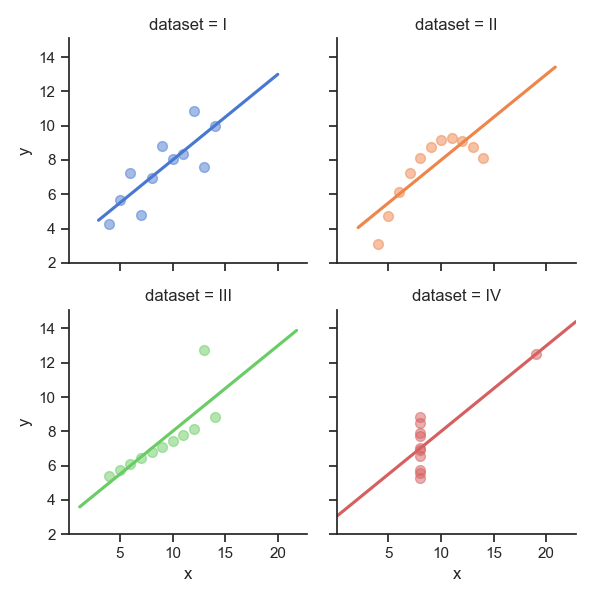
\includegraphics[width=0.5\textwidth]{test.png}
  
  \caption{\color{Gray} \textbf{A-F}, This figure is wrapped into the standard floating environment.}
  \label{fig2} % \label works only AFTER \caption within figure environment

\end{figure}

\subsection*{{\bfseries\sffamily } Figure 2 Example of a wide figure}
\label{sec:orgd82e196}
\vspace{.5cm} % set vertical space between text and figure
\begin{adjustwidth}{-2.25in}{0in}

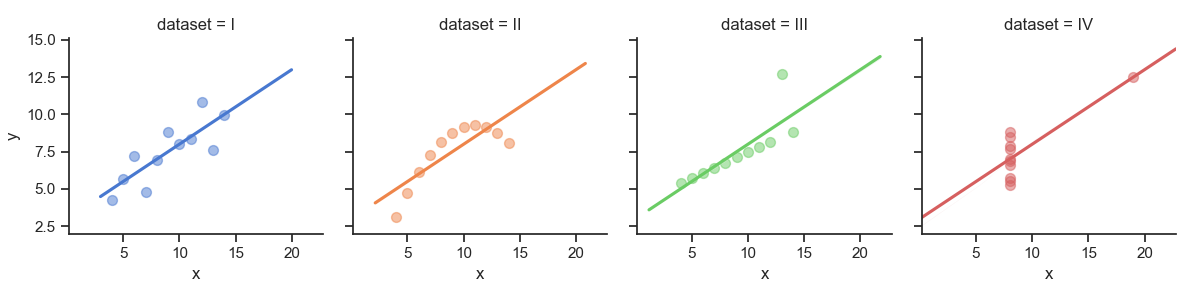
\includegraphics[width=163mm]{test2.png}

\justify 
\color{Gray}
% do not use '\caption outside of a float
\small{
  \textbf {Figure 2. Example of a wide figure with multi-page caption.}
  \textbf{A}, Start junk text here: Proin lectus ex, venenatis vel ornare eget, hendrerit tempus justo. Pellentesque molestie purus sed pretium tincidunt. Curabitur facilisis, orci vitae mollis fringilla, elit erat fermentum justo, nec luctus nunc sapien vel dolor. Cras enim justo, ullamcorper ut commodo at, posuere et ex. Fusce cursus sapien id augue maximus convallis. Praesent egestas massa in enim volutpat varius. In aliquam turpis urna, at elementum turpis eleifend at. \textbf{B}, Proin risus erat, tincidunt quis massa non, sollicitudin congue metus. Aliquam quis magna vulputate, posuere est eu, tempor nisi. Cras gravida tempus felis, vitae lacinia lacus volutpat quis. Pellentesque et eros eu mi suscipit tempus. Proin in augue scelerisque. \textbf{C}, Donec a tempor tortor, et dignissim enim. Cras in ipsum sed velit bibendum imperdiet. Aenean aliquet mauris maximus, sodales ligula sit amet, placerat felis. In tristique nisi eu risus rutrum, ac lacinia lorem cursus. Nunc eget condimentum purus. Maecenas imperdiet nisl eu accumsan gravida. \textbf{D}, Nullam tincidunt, magna sed auctor ultrices, leo mi eleifend velit, quis varius ex diam non tellus. Nam tincidunt vehicula turpis, ut euismod turpis elementum vel.
}
\end{adjustwidth}

Resume Results section. \lipsum[6]
\section*{{\bfseries\sffamily } Discussion}
\label{sec:orge6d0cab}
Summarize the results in the context of existing literature. \lipsum

\let\oldbibliography\thebibliography
\renewcommand{\thebibliography}[1]{\oldbibliography{#1}
  \setlength{\itemsep}{-1pt}} % Reducing spacing in the bibliography.
\footnotesize{ % https://www.sharelatex.com/learn/Font_sizes,_families,_and_styles#Reference_guide
  \bibliography{bibliography.bib} 
  \bibliographystyle{nihunsrt} % Use the custom nihunsrt bibliography style included with the template
}\normalsize
\end{document}